\chapter{Proposta de Trabalho}
\label{chap:proposta}

Neste capítulo é apresentado um plano de trabalho que será elaborado
durante o período após a qualificação, e resultados esperados.
Este trabalho tem o objetivo de trazer duas contribuições:
\begin{enumerate}
    \item Uma opção no compilador GCC para que ele seja
capaz de compilar um único arquivo em paralelo sem utilizar a
estrutura do LTO. Isso é útil para desenvolvedores que trabalham
com grandes softwares iterativamente, pois deve minimizar
gargalos gerados por arquivos grandes e cobrir os casos onde o LTO gera
binário menos eficientes que o processo clássico de compilação, fornecendo assim
uma alternativa ao LTO.
Essa tese se concentra em paralelizar os passos de otimização Intra Procedural
a nível de funções, ou seja, duas análises executarão em paralelo em funções
distintas, evitando adentrar em paralelizar a análise de fluxo de dados.

    \item Uma revisão sobre o que pode ser feito para acelerar o
processo clássico de compilação em máquinas \textit{manycore}, através
de paralelismo, e quais problemas devem ser atacados em trabalhos futuros.
Espera-se utilizar os resultados do item 1.
\end{enumerate}
O primeiro item será enviada ao GCC como como uma contribuição
ao \textit{software} livre. O projeto de paralelização foi submetido para o GSoC 2019,
conforme o Apêndice \ref{ap:gsoc}.


\section{Paralelização do GCC com \textit{threads}}

Nesta subseção é apresentado o estado atual do projeto de paralelização
do GCC com \textit{threads}. O GCC foi escolhido como candidato para
paralelização pois a comunidade demonstrou grande interesse no projeto,
conforme discutido na Seção \ref{cap:introducao}, e o autor desta tese ter alguma
familiaridade com o projeto, já tendo contribuído com este. Sendo assim,
utilizar outro compilador como o Clang para implementar o projeto demandaria
estudos sobre a estrutura do projeto e convencer parte da comunidade de que
o trabalho trás alguma vantagem ao projeto. Por outro lado, implementar um
novo compilador não é uma alternativa viável dado que um dos maiores gargalos
na compilação é o otimizador, peça que não seria possível implementar em
dois anos algo tão poderoso como o GCC ou o Clang.

Como atestado por \cite{PR84402}, há um gargalo de paralelismo dentro do
próprio GCC por conta de arquivos grandes, e \cite{mailgcc} também
relatou um gargalo em outro projeto interno. Uma das soluções para este
problema é melhorar o paralelismo dentro do GCC, tornando possível fazer
com que a compilação utilize mais núcleos de processamento.
Nesta discussão, foi proposto uma maneira de visualizar o problema de
paralelismo através de um gráfico gerado por dados de um GNU Make modificado.
Como a alteração no Make é razoavelmente complicada e o \textit{script} proposto
havia sérios problemas de estabilidade, foi desenvolvido uma outra maneira
de replicar os resultados.

Como desenvolvido e publicado por \cite{gcctimer}, a ferramenta aqui proposta
é capaz de coletar e exibir dados referente ao tempo de compilação
de cada arquivo no GCC, incluindo os testes gerados pelo GNU Autotools.
A ferramenta funciona da seguinte forma: há um programa escrito em C chamado
\texttt{cc\_wrapper} que encapsula o compilador C e C++ do ambiente, no caso o 
GCC e o G++. O caminho para estes compiladores são passados como um parâmetro
da compilação do \texttt{cc\_wrapper} de maneira que os binários gerados os
simulem. Em seguida o programa abre um novo processo através do \texttt{fork()},
chamando o GCC/G++ com os parâmetros passados a ele sem alterações. O processo
inicia a coleta do tempo, busca pelo nome do arquivo objeto a ser gerado, e
aguarda o GCC chamado terminar. Essa busca foi codificada de maneira a ser
muito eficiente, tento um pior caso $O(n)$ com uma constante muito baixa,
onde $n$ é o número de parâmetros passados ao GCC. Em seguida, o programa
escreve o tempo de início, tempo de fim, e o nome do arquivo em um arquivo
de texto. Houve cautela para que não haja mistura de linhas
no arquivo por razão de escrita simultânea no arquivo. Há também um \textit{script}
em \textit{Bash} para reproduzir os resultados facilmente.

Em seguida, foi codificado um programa em \textit{Python} para análise dos
resultados. Esse programa é responsável por gerar os gráficos conforme
mostrado na Figura \ref{fig:analysis_classical}. Em um dos eixos há o
tempo de execução, no outro há
o trabalho do Makefile. Para construir o gráfico, é considerado que
dois intervalos que se interseccionam apenas podem ser executados em
trabalhos distintos do Make, sendo assim é utilizado a técnica
de coloração em grafos de intervalos, que pode ser resolvido otimamente
em $O(n \log p)$, onde $n$ é o número de arquivos e $p$ é o número de
cores, embora o algoritmo
implementado seja $O(np)$.

\subsection{Inverstigação do Tempo Consumido na Compilação}

Uma investigação foi conduzida com a finalidade de encontrar o gargalo
principal no processo de compilação do GCC. Todos os testes efetuados foram
executados em um computador com um AMD Opteron 6376 (64 núcleos) executando
o Debian 9.

Novamente na Figura \ref{fig:analysis_classical}, é possível notar dois
itens, independente da quantidade de execuções do experimento:

\begin{itemize}
    \item A existência de arquivos como o \texttt{gimple-match.c}, que
        geram um gargalo no paralelismo do GCC.

    \item Várias etapas sequênciais executadas pelo GNU Autoconf.
\end{itemize}

O arquivo \texttt{gimple-match.c} é gerado automaticamente compilando
o arquivo \texttt{match.pd} para C. Na versão 9.0.1 do GCC, o arquivo
gerado contém exatamente 99329 linhas de código. Espera-se que o tempo
de compilação do \texttt{gimple-match.c} diminua, em conjunto com o tempo
total de compilação, ao paralelizar o GCC com \textit{threads}.

Analisando o tempo necessário para compilar o arquivo \texttt{gimple-match.c},
foi possível notar que:
\begin{itemize}
    \item São necessários em média 76 segundos para compilar tal arquivo.

    \item 91\% desse tempo (69 segundos) são utilizados na etapa de otimização
        e geração de código final.

    \item 8\% desse tempo (6 segundos) são utilizados na etapa de análise léxica
        e sintática.

    \item O outro 1\% está distribuído em diversas partes do compilador.
\end{itemize}
Todos estes dados foram obtidos autocompilando o GCC 9.0.1, e utilizando a
ferramenta de \textit{profiling} incorporada
no GCC através das flags \texttt{-ftime-report} \texttt{-ftime-report-details}.

Como as otimizações do GCC são divididas em IPA, GIMPLE e RTL, é necessário
executar uma granularidade mais fina na análise. Com uma simples alteração
no GCC, foi possível separar a etapa IPA das demais. Bastou embrulhar as funções
\texttt{ipa\_passes()} e \texttt{expand\_all\_functions()} com duas\textit{timevars}
distintas. Assim, os dados são:
\begin{itemize}
    \item 75\% do tempo total de compilação (57s) é gasto nos passos de otimização
        Intra Procedural e geração de código.

    \item 11\% do tempo total de compilação (11s) é gasto para realizar as IPA.
\end{itemize}
Sendo assim, o principal candidato a paralelização é a função \texttt{expand\_all\_functions()}.
Entretanto, para realizar tal paralelização, será necessário documentar e remover diversas
variáveis globais do GCC de maneira que seja possível realizar paralelismo com \textit{threads}.

\subsection{Análise do \textit{Speedup} Máximo}

Conforme analisado acima, se paralelizarmos as etapas de otimização Intra
Procedural e Geração de Código, é possível paralelizar 75\% do tempo total.
Sendo assim, seja $p$ o número de processadores utilizados. Assumindo
\textit{speedup} linear, o ganho máximo será:

$$ T_p = \frac{1}{4} T_1 + \frac{3}{4p}T_1 = \frac{1}{4} \left( 1 + \frac{3}{p}
\right)T_1 $$ Sendo assim, o \textit{speedup} máximo por arquivo será: $$
\lim_{p \rightarrow +\infty} \frac{T_1}{T_p} = \lim_{p \rightarrow +\infty}
\frac{T_1}{\frac{1}{4} \left( 1 + \frac{3}{p} \right)T_1} = \lim_{p \rightarrow
+\infty} \frac{4}{1 + \frac{3}{p}} = 4$$
Entretanto, é muito provável que o \textit{speedup} a ser obtido seja menor que isto
devido a mecanismos de sincronização necessários para implementar o paralelismo.

\subsection{Experimentos e Metodologia}

Para validar os resultados obtidos, serão executados dois experimentos:
\begin{enumerate}
    \item Comparação do tempo de compilação do arquivo \texttt{gimple-match.c}
        antes e após a paralelização.


    \item Comparação do tempo total de compilação do GCC antes e após a paralelização.
\end{enumerate}
Tal comparação será realizada utilizando
técnicas de inferência estatística conforme descrito por
\cite{morettin2017estatistica}: Serão
coletadas diversas amostras, realizado alguma suposição com respeito a distribuição
do tempo de acordo com as amostras coletadas e o resultado de um gráfico Q-Q, utilizado um estimador para a variância
de acordo com a distribuição, e calculado os intervalos de confiança sobre a média
para afirmar que a média do tempo realmente diminui com a paralelização. Caso não
seja possível encontrar uma distribuição que melhor se adeque aos dados, será utilizado
o Teorema do Limite Central com um número grande de amostras no cálculo dos intervalos.
Para afirmar que o tempo realmente diminui, os intervalos de confiança não deverão
se sobrepor, e a média do tempo após a paralelização deverá ser menor que o tempo
antes da paralelização.

Para afirmar que o GCC continua correto após a paralelização, serão executados
todos os testes na suíte de testes do GCC, na qual o compilador deverá passar.
No caso de falha de poucos testes, será averiguado a causa da falha. Se atestado
que o problema é de fato o teste, então este será atualizado para
esperar o paralelismo do compilador.

\subsection{Cronograma}

As atividades serão dispostas pelos próximos meses na seguinte forma:

\begin{itemize}
	\item Separar GIMPLE e RTL: O RTL tem dependências com o \textit{Back End}
	do GCC, sendo assim os passos GIMPLE e RTL serão separados para que seja
	possível paralelizar os passos GIMPLE.

	\item Remover estados globais: O GCC têm muitos estados globais referentes
	aos passos GIMPLE que deverão ser adaptados para a paralelização.

	\item Paralelizar o GIMPLE: Será adicionado código para que os passos do
	GIMPLE executem em paralelo, e em seguida executar os experimentos.

	\item Avaliar a paralelização do RTL e IPA: Dependendo do ganho obtido
	na etapa anterior, será avaliado o ganho de paralelizar os passos IPA ou
	o RTL.

	\item Escrita da Tese: Tempo destinado a escrita do texto final da tese.
\end{itemize}
Uma ilustração desse calendário está representado na Figura \ref{fig:gantt}.

\begin{figure}

  \centering

  \begin{ganttchart}{2019-05}{2020-3}
    \gantttitlecalendar{year,month=shortname} \ganttnewline
    \ganttgroup[progress=50]{Paralelização do GIMPLE}{2019-05}{2019-09} \ganttnewline
    \ganttbar[progress=0]{Separar GIMPLE e RTL}{2019-05}{2019-05} \ganttnewline
    \ganttbar[progress=0]{Remover estados Globais}{2019-05}{2019-07} \ganttnewline
    \ganttbar[progress=0]{Paralelizar o GIMPLE}{2019-07}{2019-09} \ganttnewline
    \ganttmilestone{Experimentos}{2019-09} \ganttnewline
    \ganttgroup[progress=30]{Avaliar a paralelização do RTL e IPA}{2019-10}{2019-12} \ganttnewline
    \ganttgroup[progress=20]{Escrita da Tese}{2019-12}{2020-02} \ganttnewline
    \ganttmilestone{Submissão}{2020-02}
  \end{ganttchart}

  \caption{Cronograma das Atividades.\label{fig:gantt}}
\end{figure}



\begin{figure}[ht]
 \centering
 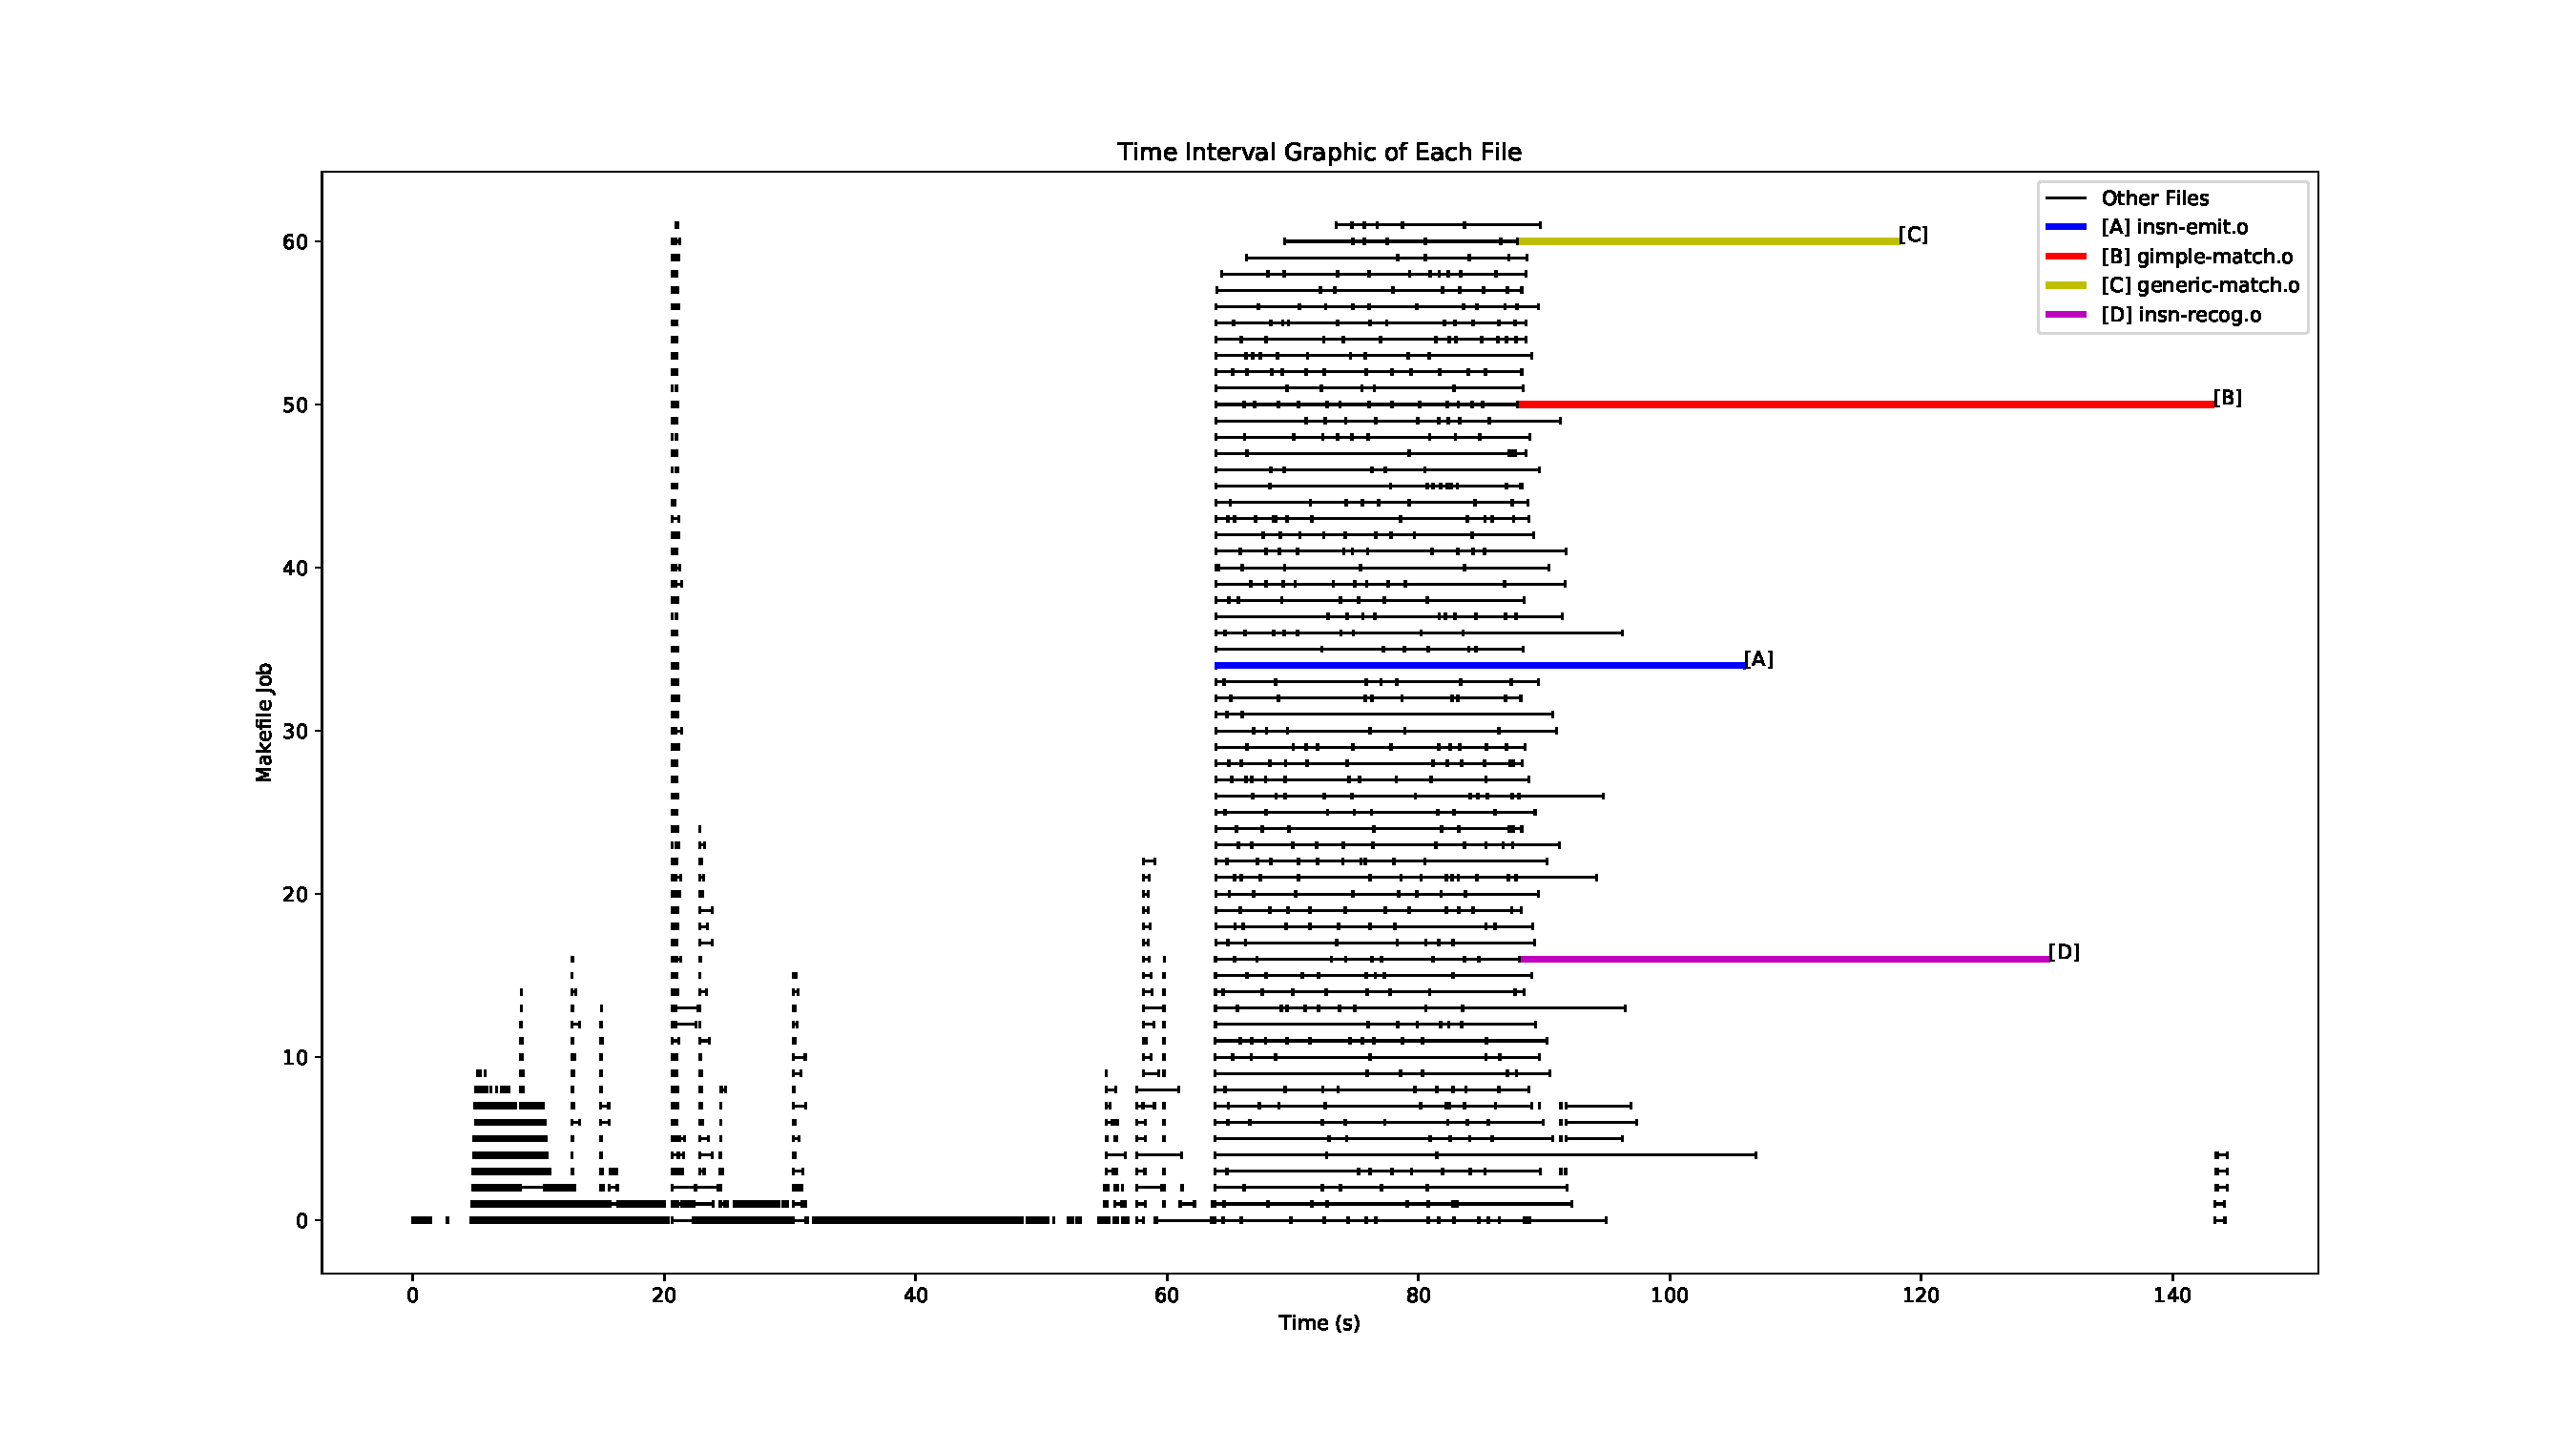
\includegraphics[scale=0.6, angle=-90]{gcc_timer_classic.pdf}
 \caption{Tempo corrido na compilação do GCC em um processador de 64 núcleos. Sem \textit{Bootstrap}}
 \label{fig:analysis_classical}
\end{figure}


%%%%%
